\documentclass[12pt]{article}
\usepackage[utf8]{inputenc}

\usepackage{lmodern}

\usepackage{enumitem}
\usepackage[margin=2cm]{geometry}

\usepackage{amsmath, amsfonts, amssymb}
\usepackage{graphicx}
%\usepackage{subfigure}
\usepackage{tikz}
\usepackage{pgfplots}
\usepackage{multicol}

\usepackage{comment}
\usepackage{url}
\usepackage{calc}
\usepackage{subcaption}
\usepackage[indent=0pt]{parskip}
\usepackage{animate}

\usepackage{array}
\usepackage{blkarray,booktabs, bigstrut}
\usepackage{bigints}

\pgfplotsset{compat=1.16}

% MATH commands
\newcommand{\ga}{\left\langle}
\newcommand{\da}{\right\rangle}
\newcommand{\oa}{\left\lbrace}
\newcommand{\fa}{\right\rbrace}
\newcommand{\oc}{\left[}
\newcommand{\fc}{\right]}
\newcommand{\op}{\left(}
\newcommand{\fp}{\right)}

\newcommand{\bi}{\mathbf{i}}
\newcommand{\bj}{\mathbf{j}}
\newcommand{\bk}{\mathbf{k}}
\newcommand{\bF}{\mathbf{F}}

\newcommand{\mR}{\mathbb{R}}

\newcommand{\ra}{\rightarrow}
\newcommand{\Ra}{\Rightarrow}

\newcommand{\sech}{\mathrm{sech}\,}
\newcommand{\csch}{\mathrm{csch}\,}
\newcommand{\curl}{\mathrm{curl}\,}
\newcommand{\dive}{\mathrm{div}\,}

\newcommand{\ve}{\varepsilon}
\newcommand{\spc}{\vspace*{0.5cm}}

\DeclareMathOperator{\Ran}{Ran}
\DeclareMathOperator{\Dom}{Dom}

\newcommand{\exo}[1]{\noindent\textcolor{red}{\fbox{\textbf{Problem {#1}}}\hrulefill}\\\\ }
\newcommand{\qu}[4]{\noindent\textcolor{#4}{\fbox{\textbf{Section {#1} | Problem {#2}}} \hrulefill{{\fbox{\textbf{{#3} Points}}}}\\}}

\newcommand{\semester}{Fall 2023}

\newcommand{\CVup}{%

\begin{tikzpicture}
\draw[black, <->, >=latex] (-0.33, 0.5) .. controls (-0.125, 0) and (0.125, 0) .. (0.33, 0.5);
\end{tikzpicture}}

\newcommand{\CVupInc}{%
\begin{tikzpicture}
\draw[black, ->, >=latex] (0,0) .. controls (0.2, 0) and (0.4, 0.2) .. (0.5, 0.5);
\end{tikzpicture}}

\newcommand{\CVupDec}{%
\begin{tikzpicture}[rotate=270]
\draw[black, ->, >=latex] (0,0) .. controls (0.2, 0) and (0.4, 0.2) .. (0.5, 0.5);
\end{tikzpicture}}

\newcommand{\CVdown}{%
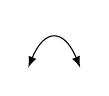
\begin{tikzpicture}
\draw[black, <->, >=latex] (-0.33, -0.5) .. controls (-0.125, 0) and (0.125, 0) .. (0.33, -0.5);
\end{tikzpicture}}

\newcommand{\CVdownInc}{%
\begin{tikzpicture}
\draw[black, ->, >=latex] (-0.5, -0.5) .. controls (-0.5, -0.3) and (-0.5, -0.1) .. (0,0);
\end{tikzpicture}}

\newcommand{\CVdownDec}{%
\begin{tikzpicture}[rotate=-90]
\draw[black, ->, >=latex] (-0.5, -0.5) .. controls (-0.5, -0.3) and (-0.5, -0.1) .. (0,0);
\end{tikzpicture}}

\begin{document}
	\noindent \hrulefill \\
	MATH-244 \semester \hfill Practice Problems Solutions\\
	Section 15.8 \hfill Pierre-Olivier Paris{\'e} \\\vspace*{-1cm}
	
	\noindent\hrulefill
	
	\spc	

	\exo{8}
	\\
	Since $\rho = \sqrt{x^2 + y^2 + z^2}$ and $\cos \phi = z/\rho = z/\sqrt{x^2 + y^2 + z^2}$. Combining everything together gives the following equation:
		\begin{align*}
		\sqrt{x^2 + y^2 + z^2} = \frac{z}{\sqrt{x^2 + y^2 + z^2}} \quad \Ra \quad x^2 + y^2 + z^2 = z .
		\end{align*}
	So, rewritting the last equation in the following way:
		\begin{align*}
		x^2+ y^2 + (z - 1/2)^2 = 1/4, 
		\end{align*}
	we see that the surface is a sphere of radius $1/2$ and centered at $(0, 0, 1/2)$.
	
	\spc

	\exo{26}
	\\
	The equation of the cone is $\phi = \pi/4$ because
		\begin{align*}
		z = \sqrt{x^2 + y^2} \iff \phi = \pi/4 .
		\end{align*}
	The equation of the first sphere is $\phi = 1$ and the equation of the second sphere is $\rho = 2$. So the solid can be described in spherical coordinates as followed:
		\begin{align*}
		E = \{ (\rho , \theta , \phi ) \, : \, 1 \leq \rho \leq 2 , 0 \leq \theta \leq 2 \pi , 0 \leq \phi \leq \pi/4 \} .
		\end{align*}
	
	Using the change of variable formula for spherical coordinates, we obtain
		\begin{align*}
		\iiint_E \sqrt{x^2 + y^2 + z^2} \, dV &= \int_0^{\pi/4} \int_{0}^{2\pi} \int_1^2 \rho^3 \sin (\phi ) \, d\rho d\theta d\phi \\
		&= \Big( \int_0^{\pi/4} \sin \phi \, d\phi \Big) \Big( \int_0^{2\pi} \, d\theta \Big) \Big( \int_1^2 \rho^3 \, d\rho \Big) \\
		&= (1-1/\sqrt{2}) (2\pi) (15/4) = (\sqrt{2} - 1) 15 \pi /(2\sqrt{2}) .
		\end{align*}
	
	\spc
	
	\exo{30}
	\\
	The volume of the solid $E$ is given by
		\begin{align*}
		V (E) = \iiint_E 1 \, dV = \iiint_E \, dV .
		\end{align*}
	
	The solid lies below the cone $z = \sqrt{x^2 + y^2}$ whose equation in spherical coordinates is $\phi = \pi/4$. Since we want the portion below this cone, the angle $\phi$ is between $\phi/4$ and $\phi/2$ ($\pi/4 \leq \phi \leq \pi/2$). The equation of the sphere is simply $\rho = 2$. So the description of $E$ in spherical coordinates is
		\begin{align*}
		E = \{ (\rho , \theta , \phi ) \, : \, 0 \leq \rho \leq 2 , 0 \leq \theta \leq 2\pi , \pi/4 \leq \phi \leq \pi/2 \} .
		\end{align*}
		
	Now, using the change of variable formular for spherical coordinates, the volume of $E$ is given by
		\begin{align*}
		V (E) &= \int_{\pi/4}^{\pi/2} \int_0^{2\pi} \int_0^2 \rho^2 \sin (\phi ) \, d\rho d \theta d \phi \\
		&= \Big( \int_{\pi/4}^{\pi/2} \sin \phi \, d\phi \Big) \Big( \int_0^{2\pi} \, d\theta \Big) \Big( \int_0^2 \rho^2 \, d \rho \Big)\\
		&= (1/\sqrt{2})(2\pi) (8/3) = 16\pi/(3\sqrt{2}) .
		\end{align*}

\end{document}